\documentclass[11pt]{book}

%%%%%%%%%%%%%%Include Packages%%%%%%%%%%%%%%%%%%%%%%%%%%
\usepackage{xcolor}
\usepackage{mathtools}
\usepackage[legalpaper, total={6in, 8in}, margin=1.25in]{geometry}
\usepackage{amsmath}
\usepackage{amssymb}
\usepackage{paralist}
\usepackage{rsfso}
\usepackage{amsthm}
\usepackage{wasysym}
\usepackage[inline]{enumitem}   
\usepackage{hyperref}
\usepackage{tocloft}
\usepackage{wrapfig}
\usepackage{titlesec}
\usepackage{colortbl}
\usepackage{stackengine} 
\usepackage{csvsimple}
\usepackage{listings}
%%%%%%%%%%%%%%%%%%%%%%%%%%%%%%%%%%%%%%%%%%%%%%%%%%%%%%%%



%%%%%%%%%%%%%%%Code%%%%%%%%%%%%%%%%%%%%%%%%%%%%%%%%%%%%%
\definecolor{codegreen}{rgb}{0,0.6,0}
\definecolor{codegray}{rgb}{0.5,0.5,0.5}
\definecolor{codepurple}{rgb}{0.58,0,0.82}
\definecolor{backcolour}{rgb}{0.95,0.95,0.92}

\lstdefinestyle{mystyle}{
    backgroundcolor=\color{backcolour},   
    commentstyle=\color{codegreen},
    keywordstyle=\color{magenta},
    numberstyle=\tiny\color{codegray},
    stringstyle=\color{codepurple},
    basicstyle=\ttfamily\footnotesize,
    breakatwhitespace=false,         
    breaklines=true,                 
    captionpos=b,                    
    keepspaces=true,                 
    numbers=left,                    
    numbersep=5pt,                  
    showspaces=false,                
    showstringspaces=false,
    showtabs=false,                  
    tabsize=2
}
%%%%%%%%%%%%%%%%%%%%%%%%%%%%%%%%%%%%%%%%%%%%%%%%%%%%%%%%




%%%%%%%%%%%%%%%Chapter Setting%%%%%%%%%%%%%%%%%%%%%%%%%%
\definecolor{gray75}{gray}{0.75}
\newcommand{\hsp}{\hspace{20pt}}
\titleformat{\chapter}[hang]{\Huge\bfseries}{\thechapter\hsp\textcolor{gray75}{$\mid$}\hsp}{0pt}{\Huge\bfseries}
%%%%%%%%%%%%%%%%%%%%%%%%%%%%%%%%%%%%%%%%%%%%%%%%%%%%%%%%

%%%%%%%%%%%%%%%%%Theorem environments%%%%%%%%%%%%%%%%%%%
\newtheoremstyle{break}
  {\topsep}{\topsep}%
  {\itshape}{}%
  {\bfseries}{}%
  {\newline}{}%
\theoremstyle{break}
\theoremstyle{break}
\newtheorem{axiom}{Axiom}
\newtheorem{thm}{Theorem}[section]
\renewcommand{\thethm}{\arabic{section}.\arabic{thm}}
\newtheorem{lem}{Lemma}[thm]
\newtheorem{prop}[lem]{Proposition}
\newtheorem{corL}{Corollary}[lem]
\newtheorem{corT}[lem]{Corollary}
\newtheorem{defn}{Definition}[corL]
\newenvironment{indEnv}[1][Proof]
  {\proof[#1]\leftskip=1cm\rightskip=1cm}
  {\endproof}
%%%%%%%%%%%%%%%%%%%%%%%%%%%%%%%%%%%%%%%%%%%%%%%%%%%%%%


%%%%%%%%%%%%%%%%%%%%%%%Integral%%%%%%%%%%%%%%%%%%%%%%%
\def\upint{\mathchoice%
    {\mkern13mu\overline{\vphantom{\intop}\mkern7mu}\mkern-20mu}%
    {\mkern7mu\overline{\vphantom{\intop}\mkern7mu}\mkern-14mu}%
    {\mkern7mu\overline{\vphantom{\intop}\mkern7mu}\mkern-14mu}%
    {\mkern7mu\overline{\vphantom{\intop}\mkern7mu}\mkern-14mu}%
  \int}
\def\lowint{\mkern3mu\underline{\vphantom{\intop}\mkern7mu}\mkern-10mu\int}
%%%%%%%%%%%%%%%%%%%%%%%%%%%%%%%%%%%%%%%%%%%%%%%%%%%%%%



\newcommand{\R}{\mathbb{R}}
\newcommand{\N}{\mathbb{N}}
\newcommand{\Z}{\mathbb{Z}}
\newcommand{\Q}{\mathbb{Q}}
\newcommand{\C}{\mathbb{C}}
\newcommand{\T}{\mathcal{T}}
\newcommand{\M}{\mathcal{M}}
\newcommand{\Symm}{\text{Symm}}
\newcommand{\Alt}{\text{Alt}}
\newcommand{\Int}{\text{Int}}
\newcommand{\Bd}{\text{Bd}}
\newcommand{\Power}{\mathcal{P}}
\newcommand{\ee}[1]{\cdot 10^{#1}}
\newcommand{\spa}{\text{span}}
\newcommand{\sgn}{\text{sgn}}
\newcommand{\degr}{\text{deg}}
\newcommand{\pd}{\partial}
\newcommand{\that}[1]{\widetilde{#1}}
\newcommand{\lr}[1]{\left(#1\right)}
\newcommand{\vmat}[1]{\begin{vmatrix} #1 \end{vmatrix}}
\newcommand{\bmat}[1]{\begin{bmatrix} #1 \end{bmatrix}}
\newcommand{\pmat}[1]{\begin{pmatrix} #1 \end{pmatrix}}
\newcommand{\rref}{\xrightarrow{\text{row\ reduce}}}
\newcommand{\txtarrow}[1]{\xrightarrow{\text{#1}}}
\newcommand\oast{\stackMath\mathbin{\stackinset{c}{0ex}{c}{0ex}{\ast}{\Circle}}}


\newcommand{\note}{\color{red}Note: \color{black}}
\newcommand{\remark}{\color{blue}Remark: \color{black}}
\newcommand{\example}{\color{green}Example: \color{black}}
\newcommand{\exercise}{\color{green}Exercise: \color{black}}

%%%%%%%%%%%%%%%%%%%%%%Roman Number%%%%%%%%%%%%%%%%%%%%%%%
\makeatletter
\newcommand*{\rom}[1]{\expandafter\@slowromancap\romannumeral #1@}
\makeatother
%%%%%%%%%%%%%%%%%%%%%%%%%%%%%%%%%%%%%%%%%%%%%%%%%%%%%%%%%

%%%%%%%%%%%%table of contents%%%%%%%%%%%%%%%%%%%%%%%%%%%%
\setlength{\cftchapindent}{0em}
\cftsetindents{section}{2em}{3em}

\renewcommand\cfttoctitlefont{\hfill\huge\bfseries}
\renewcommand\cftaftertoctitle{\hfill\mbox{}}

\setcounter{tocdepth}{2}
%%%%%%%%%%%%%%%%%%%%%%%%%%%%%%%%%%%%%%%%%%%%%%%%%%%%%%%%%


%%%%%%%%%%%%%%%%%%%%%Footnotes%%%%%%%%%%%%%%%%%%%%%%%%%%%
\newcommand\blfootnote[1]{%
  \begingroup
  \renewcommand\thefootnote{}\footnote{#1}%
  \addtocounter{footnote}{-1}%
  \endgroup
}
%%%%%%%%%%%%%%%%%%%%%%%%%%%%%%%%%%%%%%%%%%%%%%%%%%%%%%%%%

%%%%%%%%%%%%%%%%%%%%%Section%%%%%%%%%%%%%%%%%%%%%%%%%%%%%
\makeatletter
\def\@seccntformat#1{%
  \expandafter\ifx\csname c@#1\endcsname\c@section\else
  \csname the#1\endcsname\quad
  \fi}
\makeatother
%%%%%%%%%%%%%%%%%%%%%%%%%%%%%%%%%%%%%%%%%%%%%%%%%%%%%%%%%

%%%%%%%%%%%%%%%%%%%%%%%%%%%%%%%%%%%Enumerate%%%%%%%%%%%%%%
\makeatletter
% This command ignores the optional argument 
% for itemize and enumerate lists
\newcommand{\inlineitem}[1][]{%
\ifnum\enit@type=\tw@
    {\descriptionlabel{#1}}
  \hspace{\labelsep}%
\else
  \ifnum\enit@type=\z@
       \refstepcounter{\@listctr}\fi
    \quad\@itemlabel\hspace{\labelsep}%
\fi}
\makeatother
\parindent=0pt
%%%%%%%%%%%%%%%%%%%%%%%%%%%%%%%%%%%%%%%%%%%%%%%%%%%%%%%%%%


\begin{document}

	\begin{titlepage}
		\begin{center}
			\vspace*{1cm}
			\Huge \color{red}
				\textbf{Lab 2 Report}\\
			\vspace{0.5cm}			
			\Large \color{black}
				Math 391 - Introduction to Modern Physics Lab\\
				Professor Wayne Lau\\	
				University of Michigan\\
			\vspace{3cm}

			
\includegraphics[scale=1.16]{Jinyan'sPortrait.pdf}
			
			
			\vspace{5cm}
			\LARGE
				\textbf{Jinyan Miao}\\
				\hfill\break
				\LARGE Fall 2022\\
			\vspace{1cm}

		\vspace*{\fill}
		\end{center}			
	\end{titlepage}


\newpage
\tableofcontents
\addtocontents{toc}{~\hfill\textbf{Page}\par}


\setcounter{chapter}{2}
\chapter*{Lab 2 - Blackbody Radiation}
\section{Introduction}
In the early 20th century, British physicist Lord Rayleigh derived the Rayleigh-Jeans law through classical arguments and empirical facts: 
\begin{align*}
\frac{dI}{df} = \frac{2\pi f^2}{c^2}\, kT \tag{Rayleigh-Jeans law}
\end{align*}
The Rayleigh-Jeans law, which approximates spectral radiance of electromagnetic radiation as a function of wavelength and temperature, agrees with experimental results for large wavelengths, but it diverges for short wavelengths, which leads to the so-called UV catastrophe. The resolution to the UV catastrophe was given by Max Planck of Planck's law for blackbody radiation, which assumes the quantization of photon energy, and that gives the correct result for blackbody radiation at both long and short wavelengths:
\begin{align}
\frac{dI}{df} = \frac{2\pi hf^3}{c^2}\frac{1}{e^{hf/(kT)}-1}
\end{align} 
Planck's result also suggests that the intensity radiated by the blackbody is proportional to $T^4$ with a constant of proportionality $\sigma_s$, which agrees with the Stefan–Boltzmann law that was experimentally verified in the late 19th century: 
\begin{align}
I = \sigma_s\, T^4
\end{align}
In Lab 2 of Physics 391, we verify the $T^4$ dependence of the radiation intensity, and we demonstrate the spectral intensity temperature dependence. We do so by measuring the temperature and the radiated intensity of an incandescent lamp when the lamp is powered by a source, then we fit our data with (2.1) and (2.2) to conclude our results. This lab is designed to help us to develop a better understanding of Planck's law and Stefan-Boltzmann law for blackbody radiation.  

\hfill\break
\hfill\break
\newpage
\section{Experimental setup}
In this lab, we explore the properties of blackbody radiation by using a 12-volt incandescent lamp. The intensity radiated by the lamp can be approximated by measuring the power that it consumes:
\begin{align}
P = IV
\end{align}
where $I$ is the current through the lamp and $V$ is the voltage across the lamp. The temperature of the lamp is varied by changing the voltage across the lamp, and calculated from the effective resistance of the lamp.\\

The Lab consists of two parts. In the first part, we investigate the spectral intensity temperature dependence. A silicon photodiode is used for detecting the spectral intensity of the lamp at three different wavelengths, 550 nm (green), 750 nm (red), and 950 nm (dark).  Each wavelength is selected by a bandpass filter. The lamp is held in place and wired in a box, and a bandpass filter is placed between the lamp and the silicon photodiode. When the lamp is powered, the light emitted from the lamp first goes through the bandpass filter, then the intensity of the filtered light is recorded by measuring the current through the photodiode, and at the same time, the current and voltage across the lamp is measured. We repeat this process for all three bandpass filters. The temperature of the lamp is calculated through the following approximation proposed by Howard Jones and Irving Langmuir at the General Electric Corporation in 1927:
\begin{align*}
T = \frac{a+br + cr^2}{1+dr} \qquad\qquad\text{where }r=\frac{R-R_{\text{cord}}}{R_{\text{room temperature}}} \tag{T}
\end{align*} 
where $a=-4.129538\ee{-1}$, $b=4.360552\ee{-3}$, $c=7.399998\ee{-7}$, and $d =6.195380\ee{-5}$. $R = V/I$ is the resistance of the lamp measured when different voltages $V$ is applied across the lamp, $R_{\text{cord}}$ is the resistance of the power cord which we measured before performing the experiment, and $R_{\text{room temperature}}$ is the resistance of the lamp at room temperature. We measure $R_{\text{room temperature}}$ before and after the experiment to ensure the consistency of our data. We then fit our data (the ratio of temperature $T/T_{max}$ of the lamp, and the corresponding ratio of current $i/i_{max}$ through the photodiode) with the following equation to determine the filter wavelengths $\lambda$ of the bandpass filter:
\begin{align}
\log_{10}\left( \frac{i}{i_{max}}\right) = \log_{10}\left( e^{\frac{hc}{\lambda kT_{max}}} - 1\right) -\log_{10}\left(e^{\frac{hc}{\lambda kT}} - 1\right)
\end{align}  
Note that (1.4) can be derived by scaling both sides of (2.1) by the maximum intensity and then taking the logarithm.\\

The second part of the lab is measuring the radiated power of the lamp at different temperatures. In this part, we simply repeat the measure in the first part except without the bandpass filters and the photodiode. That is, we measure the current and the voltage across the lamp, and calculate the temperature and power of the lamp. Then we fit our data (the power of the lamp $P$, and the temperature $T$) to the following equation to determine the power dependence $T^4$ in the Stefan-Boltzmann law:
\begin{align}
\log(P) = m \log(T) +b
\end{align}
where $m$ should give us the theoretical value of $4$, and $b$ is a constant. Here we note that (2.5) can be obtained by taking the log of both sides of (2.2). 


\newpage
\section{Visualizing the data}
For the measurement of spectral intensity temperature dependence, we obtain the following data for the three bandpass filters, red, green, and dark:
\begin{center}
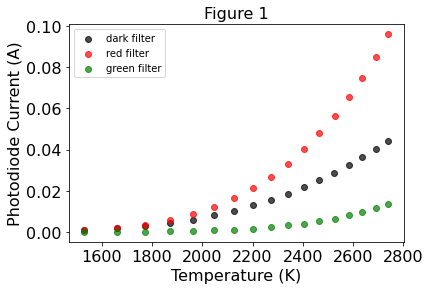
\includegraphics[scale=0.65]{IvT.png}
\end{center}
By observing Fig 1, we see that most of the energy radiated by the lamp has shorter wavelengths, as indicated by the plot that the red data points are greater than the black and green data points at a given temperature. One can also plot the log of the ratio $i/i_{max}$ of the photodiode current, over the temperature inverse $1/T$ of the lamp, as shown in the following, for the three bandpass filters:
\begin{center}
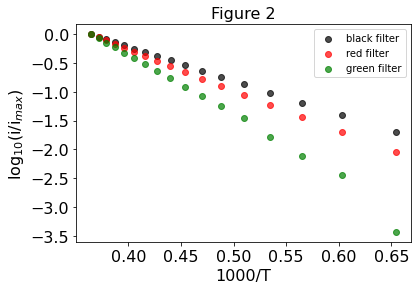
\includegraphics[scale=0.65]{logIvlogT.png}
\end{center}
Fig. 2 indicates a linear relationship between $\log(i/i_{max})$ and $1000/T$, and this relationship is predicted by (2.4) because the right-hand side of (2.4) can be approximated as a polynomial of $1/T$ with some coefficient proportional to $-hc/(\lambda k)$. That is, we write:
\begin{align}
\log\left(\frac{i}{i_{max}}\right) \propto  \frac{1}{T} \qquad\qquad\text{with proportional coefficient }-\frac{hc}{\lambda k}
\end{align}
\newpage
For the measurement of radiated power, we obtain the following data:
\begin{center}
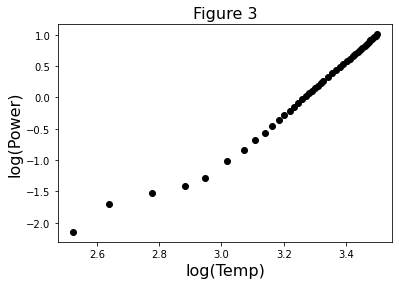
\includegraphics[scale=0.65]{logPvlogT.png}
\end{center}
where we also see an approximately linear relationship between $\log(P)$ and $\log(T)$. This relationship is predicted by (2.5), with the slope of the linear relationship given by $m$, with the theoretical value of $m=4$. \\


\newpage
\section{Analyzing the data}
First, we fit our measurement of spectral intensity temperature dependence with (2.4) to find the wavelengths $\lambda$ of the bandpass filter:
\begin{center}
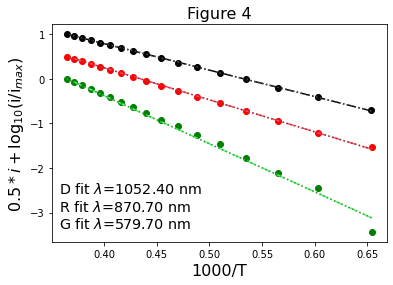
\includegraphics[scale=0.65]{fitLam.png}
\end{center}
Fig. 4 plots the data in the same way as we did in Fig. 2, except the data for the red and the dark bandpass filters are translated vertically upwards by $0.5\cdot i$, where $i=1$ for the red filter and $i=2$ for the black filter ($i=0$ for the green filter). The data are fitted before the vertical translation, and they are fitted in two different methods. The first method is minimizing the unweighted $\Delta$ quantity:
\begin{align*}
\Delta = \sum_i \left(y_i - f(x_i)\right)^2
\end{align*} 
where $f$ is the function of the model to be fitted, and $(x_i,y_i)$ is the data point. The fitted model (2.4) under this method is plotted using dash lines (-\,-). Note that the dash lines almost overlap with the dotted lines ($\cdot\ \cdot$), which represents the model fitted using the second method. For the second method, we fit the data using the scipy library function \textit{scipy.optimize.curve$\_$fit}, which fits the data using the method of non-linear squares fitting. As mentioned previously, the fitted model under the second method is plotted using the dotted lines. The error of the second method is calculated using variances. Here we note that the fitted wavelengths $\lambda$ indicated in Fig. 4 are those generated by the first method. The results of this process can be summarized by the following tables:
\hfill\break
\begin{center}
\begin{tabular}{|c|c|c|}
\hline
First method: minimizing $\Delta$ & wavelength & $\Delta$ \\ 
\hline
Green filter & 579.70\, nm & 0.1507\\
\hline
Red filter & 870.70\, nm &0.0029\\
\hline
Dark filter & 1052.40\, nm &0.0007\\
\hline
\end{tabular}\\
\hfill\break

\begin{tabular}{|c|c|c|}
\hline
Second method: minimizing variance & wavelength & Variance \\ 
\hline
Green filter & 579.66\, nm & $9.732\ee{-17}$\\
\hline
Red filter & 870.72\, nm & $9.826\ee{-18}$\\
\hline
Dark filter & 1052.39\, nm & $5.203\ee{-18}$\\
\hline
\end{tabular}
\end{center}
\hfill\break
We see that the difference between the two methods is tiny, and hence the models of the two methods almost overlap. From the slope of the models, we see that the radiated intensity for an object with a lower temperature is smaller, and by comparing the slope of the three different bandpass filters, we have verified the relationship between the radiation intensity, wavelength, and temperature of the object as characterized by (2.6), that is the slope of the lines increases as the wavelength of the bandpass filter increases. The last thing to notice here is that the wavelengths predicted by the models are about $20\%$ longer than that of the actual bandpass filters (550\, nm for green, 750\, nm for red, and 950\, nm for dark). As mentioned in the lab manual, this is most likely due to an overestimate of the filament temperature by the Jones and Langmuir model given by equation (T).\\

\newpage
For the second part of the experiment, we fit our spectral intensity data with equation (2.5).
\begin{center}
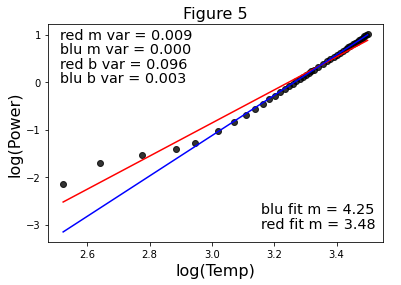
\includegraphics[scale=0.65]{radLinFit.png}
\end{center}
Fig. 5 plots the data in the same way as we did in Fig. 3. In addition we also plot two best-fit models for the data set. The first model is the red line, which is fitted by using all points in the data set. The slope of the red line is $3.48$, and the variance of parameter $m$ is  $0.009$. This indicates that the power $\alpha$ in the relationship $I = \sigma_s T^\alpha$ is around $3.48$, but this is clearly an underestimate of $m$ as we see in Fig 5. that there are some outlier data points at low temperature, which is mostly because, at low temperature, the blackbody radiation is negligible and most of the input power is dissipated by thermal conduction to the lamp filament supports and the rest of the world. By removing the first 4 data points on the left of Fig 5., we fit the rest of the data points using the blue line, and that gives us approximately zero variance for parameter $m$, with $m=4.25$. Notice that the slope of the curve $4.25$ is greater than the theoretical value of $4$, yet it is close to $4$, the difference is significant (differ by around $6\%$). Hence we are unable to conclude that the power dependence $\alpha$ in the Stefan-Boltzmann law is $4$. The cause of this result is yet to be investigated, but one possible factor is the underestimation of the temperature of the lamp by the Jones and Langmuir model given by equation (T), and the quality of the lamp might have been downgraded since its use in the first part of this lab. While we should, if we get the chance in the future, repeat the spectral intensity experiment with different lamps to get more statistical convincing results.\\



\begin{center}
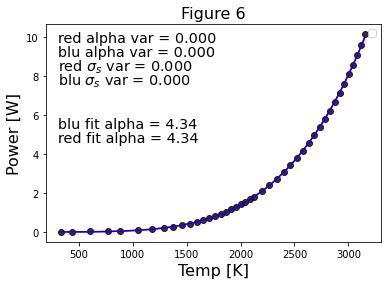
\includegraphics[scale=0.65]{radPowFit.png}
\end{center}
On the other hand, one can also fit the original data with the power law $I = \sigma_s T^{\alpha}$ to find the parameter $\alpha$. We again use the scipy library function \textit{scipy.optimize.curve$\_$fit} to obtain the model, minimizing the variance via fitting the data with parameters $\alpha$ and $\sigma_s$. The red curve in Fig. 5, which is mostly overlapped by the blue curve, is fitted using all data points in our data set. The blue curve in Fig. 5 is fitted by removing the first 4 data points at the low-temperature end. The variances for all parameters in these fittings are negligible, but we observe that the power dependence $\alpha$ is still much larger than $4$. 



\newpage
\section{Consistency of data}
Efforts have been made to ensure the consistency of the data in this experiment. Before performing the first part of this experiment (measuring spectral intensity temperature dependence), we recorded the resistance of the lamp at room temperature, and we repeat this measurement 10 minutes after the first part of the experiment. The 10 minutes period is designed to give enough time for the lamp to cool down to room temperature. We also repeat the measurement 10 minutes after the second part of the experiment (measuring the radiated power). The results are given by the following:
\begin{center}
\begin{tabular}{|c|c|c|}
\hline
& $R_{\text{room temperature}}$ & Condition of lamp \\
\hline
Before the first part & $5.129 \, \Omega$ & clear\\
\hline
After the first part & $5.135\, \Omega$ & clear \\
\hline
After the second part & $5.134\, \Omega$ & not darken\\
\hline
\end{tabular}
\end{center}
From the data recorded, we see that the condition of the lamp has not significantly changed even after the second part of the experiment. This indicates that the result we obtained should have not been affected by the quality of the lamp that we used in this experiment.\\

In addition to that, in the first part of the experiment, we start with the spectral measurements of the dark bandpass filter, and when the measurement of all three bandpass filters has been done, we repeat the spectral measurements for the dark bandpass filter. Comparing the two data sets we obtain the followings:
\begin{center}
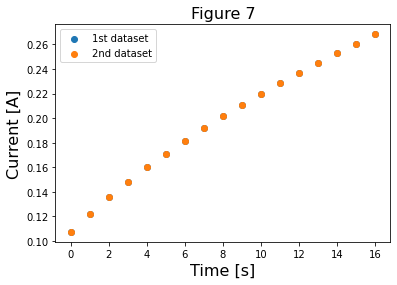
\includegraphics[scale=0.65]{comp1.png}\\
Fig. 7 Comparing the current through the lamp recorded in the two data sets\\
\hfill\break
\hfill\break
\hfill\break
\hfill\break
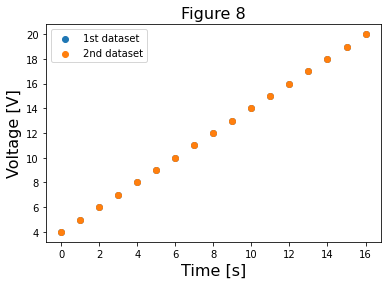
\includegraphics[scale=0.65]{comp2.png}\\
Fig. 8 Comparing the voltage across the lamp recorded in the two data sets\\
\newpage
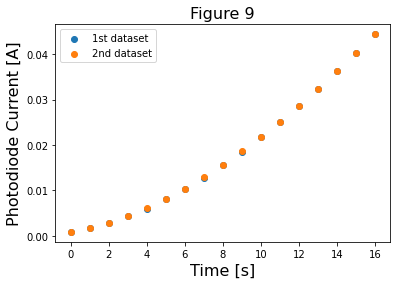
\includegraphics[scale=0.65]{comp3.png}\\
Fig. 9 Comparing the current through the photodiode recorded in the two data sets\\
\end{center}
From Fig. 7, 8, and 9, we see that the orange data points (representing the points recorded in the second data set) almost overlap with the blue data points (representing the points recorded in the first data set), which again suggests that the results in the first part of this lab should not be affected by the quality of the lamp.



\hfill\break
\hfill\break
\section{Summary}
In Lab 2 of Physics 391, we perform experiments intending to verify (I) the temperature power dependence in the Stefan-Boltzmann law, and (II) the relationship between the radiated intensity, the temperature of the blackbody, and wavelengths as revealed by Planck's law of radiation. In this text, we analyze the experiment results and conclude that (II) is well justified by our data, but we fail to verify (I) as the difference between our data and the theoretical power dependence of $\alpha = 4$ is statistically significant. We seek to perform the measurement of the radiated power of lamps again in the future to get more statistical convincing results. Nevertheless, the underlying physics in this experiment - energy of photons is quantized and hence (2.1) and (2.2) holds for blackbody radiation - is already well confirmed by many other experiments, but it is still worth spending time to experience the difficulty in generalizing those results.



\newpage
\section{Experiment Data}
\begin{center}
\begin{tabular}{|l|c|c|c|c|}%
\hline
	Black filter 1 & & & & \\
\hline	
    \bfseries Index & \bfseries Time & \bfseries Voltage &\bfseries Current & \bfseries PhotoCurrent% specify table head
    \csvreader[head to column names]{speIntB1.csv}{}% use head of csv as column names
    {\\\hline\csvcoli&\csvcolii&\csvcoliii&\csvcoliv&\csvcolv}\\% specify your coloumns here
\hline    
\hline
	Green filter 1 & & & & \\
\hline
	\bfseries Index & \bfseries Time & \bfseries Voltage &\bfseries Current & \bfseries PhotoCurrent% specify table head
    \csvreader[head to column names]{speIntG1.csv}{}% use head of csv as column names
    {\\\hline\csvcoli&\csvcolii&\csvcoliii&\csvcoliv&\csvcolv}\\% specify your coloumns here
\hline
\hline
	Red filter 1 & & & & \\
\hline
	\bfseries Index & \bfseries Time & \bfseries Voltage &\bfseries Current & \bfseries PhotoCurrent% specify table head
    \csvreader[head to column names]{speIntR1.csv}{}% use head of csv as column names
    {\\\hline\csvcoli&\csvcolii&\csvcoliii&\csvcoliv&\csvcolv}\\% specify your coloumns here
\hline
\end{tabular}

\begin{tabular}{|l|c|c|c|c|}
\hline
	Black filter 2 & & & & \\
\hline
	\bfseries Index & \bfseries Time & \bfseries Voltage &\bfseries Current & \bfseries PhotoCurrent% specify table head
    \csvreader[head to column names]{speIntB2.csv}{}% use head of csv as column names
    {\\\hline\csvcoli&\csvcolii&\csvcoliii&\csvcoliv&\csvcolv}\\% specify your coloumns here
\hline
\end{tabular}
\newpage
\hfill\break
\hfill\break
\begin{tabular}{|l|c|c|c|}
\hline
	Radiated Power & & & \\
\hline
	\bfseries Index & \bfseries Time & \bfseries Voltage &\bfseries Current % specify table head
    \csvreader[head to column names]{radPower.csv}{}% use head of csv as column names
    {\\\hline\csvcoli&\csvcolii&\csvcoliii&\csvcolv}\\% specify your coloumns here
\hline
\end{tabular}
\end{center}
\newpage

\section{Code}
The code for computing statistics of the data sets is attached.
\lstset{style=mystyle}
\lstinputlisting[language=Python]{code.py}


\end{document}